\section{Results}
\label{sec:results}
\subsection{Javascript APIs}

\begin{figure*}[t]
  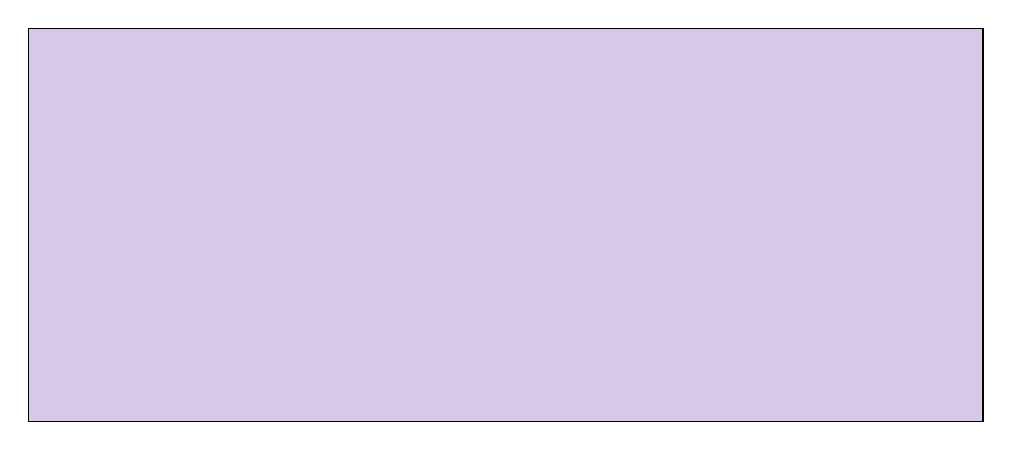
\begin{tikzpicture}
    \node[draw, fill=RoyalPurple!20, minimum width=\textwidth, minimum height=5cm] {};
  \end{tikzpicture}
  \caption{Server-side and Client-side cloaking over time}
  \label{fig:cloaking}
  \Description["TODO: "]{"TODO"}
\end{figure*}

\subsubsection{Fingerprinting APIs}{}


 
\begin{itemize}
    \item Crypto.getRandomValues jumped from SMA of 20\% to 80\% of the daily traffic (184 domains to 810) February 8th 2024
    \item The usage of seed APIs used by Su at el. (well know APIs that trackers use) has been steadily decreasing from ~30\% of the daily traffic to 15\%.
    \begin{figure}[t]
  
\begin{tikzpicture}
    \node[draw, fill=violet, minimum width=8cm, minimum height=5cm] {};
  \end{tikzpicture}
  \caption{Crypto.getRandomValues API call over time}
  \label{fig:crypto_overview}
\end{figure}
    
\end{itemize}
\subsubsection{MDN API groups over time}{}
\subsubsection{Experimental APIs and WASM}{}
\subsubsection{Fingerprintability of Kits}{}
\subsubsection{Interactive JS logs}{}
\subsubsection{Client-side cloaking tactics}{}
\subsubsection{First Party/Third Party embedded/Third Party Scripts}
\subsection{Kit families}{}
\subsubsection{Offline evaluation of detectors}{}
\subsubsection{Kit fragments and inheritence}{}
\subsubsection{First Party script fragments and inheritance}{}
\subsection{Kit detection}
\subsubsection{Kit detection via javascript}{}
\section{Case studies}
\subsection{Open Source client components}
\subsection{Mobile targets}
\subsection{Comparison to target pages}{}
